\section{Implementierung des SmBasicNetworkFailureUnlimitedRetries}

Der SmBasicNetworkFailureUnlimitedRetries baut auf das Konzept des vorherigen DEAs SmBasicSafeRetries auf. Es hat sich gezeigt, dass der Anteil der erfolgreichen Sagas erhöht werden kann, indem auf Netzwerkfehler per Forwardrecovery reagiert wird. Das Ziel dieses DEAs ist, den Anteil der vorzeitig abgebrochenen Sagas zu erhöhen. Dafür werden für die Ts \textit{BlockArticles}, \textit{RemoveMoney}, \textit{AddMoney} und \textit{StartShipment} sowie für die zugehörigen Cs ein Retry für Netzwerkfehler eingeführt. Es entsteht der DEA in \cref{fig:SmBasicNetworkfailureUnlimitedRetries}.

\begin{figure}[h!]
	\centering
	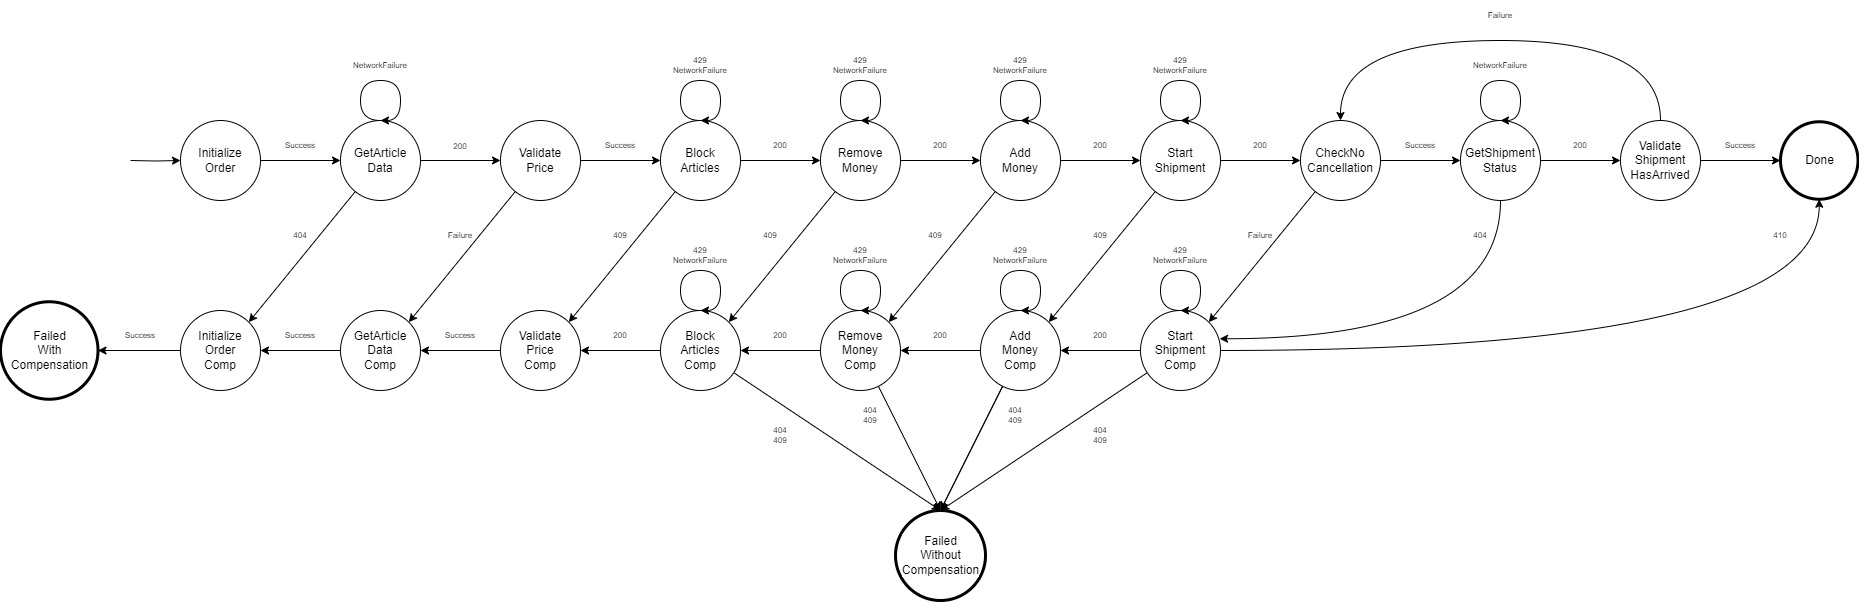
\includegraphics[width=\linewidth]{figures/ChapterVersuchsdurchführung/sm_basic_unlimited_retries.jpg}
	\caption{DEA für SmBasicNetworkfailureUnlimitedRetries}
	\label{fig:SmBasicNetworkfailureUnlimitedRetries}
\end{figure}
\FloatBarrier

\subsection{StateAnalysisResult}

Das StateAnalysisResult zeigt, dass das Einführen von Retries für transaktionelle Zustände dazu führt, dass der gewünschte Endzustand öfter erreicht wird. Testszenario 3 enthält in Testfall FinishOrders 90\% und in Testfall CancelOrders 74\% erfolgreiche Testinstanzen. Aus Sicht des Koordinators kann auf Netzwerkfehler mit einem Retry erfolgreich reagiert werden, um zum nächsten Zustand zu gelangen.

\paragraph*{Testfall FinishOrders}

\begin{center}
	\fontsize{9}{12}\selectfont
	\begin{longtable}[h]{|p{5cm}|p{1cm}|p{1cm}|p{1cm}|}
		\hline
		Messwert & S1 & S2 & S3 \\ \hline
		\endhead
		%\label{tab:smbasic_stateanalysisresult_finishorders}
		\endfoot
		successfull\-Percentage & 1.0 & 1.0 & 0.91 \\ \hline
		finished\-Percentage & 1.0 & 1.0 & 1.0 \\ \hline
		pending\-Percentage & 0.0 & 0.0 & 0.0 \\ \hline
		failedWithCompensation\-Percentage & 0.0 & 0.0 & 0.0 \\ \hline
		failedWithoutCompensation\-Percentage & 0.0 & 0.0 & 0.1 \\ \hline
		hasCorrectEndstate\-Percentage & 1.0 & 1.0 & 0.91 \\ \hline
		containsAllExpectedLogs\-Percentage & 1.0 & 1.0 & 0.91 \\ \hline
		isSuccessfullTestInstance\-Percentage & 1.0 & 1.0 & 0.91 \\ \hline
	\end{longtable}
\end{center}
\FloatBarrier

\paragraph*{Testfall CancelOrders}

\begin{center}
	\fontsize{9}{12}\selectfont
	\begin{longtable}[h]{|p{5cm}|p{1cm}|p{1cm}|p{1cm}|}
		\hline
		Messwert & S1 & S2 & S3 \\ \hline
		\endhead
		%\label{tab:smbasic_stateanalysisresult_finishorders}
		\endfoot
		successfull\-Percentage & 0.0 & 0.0 & 0.0 \\ \hline
		finished\-Percentage & 1.0 & 1.0 & 1.0 \\ \hline
		pending\-Percentage & 0.0 & 0.0 & 0.0 \\ \hline
		failedWithCompensation\-Percentage & 1.0 & 1.0 & 0.74 \\ \hline
		failedWithoutCompensation\-Percentage & 0.0 & 0.0 & 0.27 \\ \hline
		hasCorrectEndstate\-Percentage & 1.0 & 1.0 & 0.74 \\ \hline
		containsAllExpectedLogs\-Percentage & 1.0 & 1.0 & 0.74 \\ \hline
		isSuccessfullTestInstance\-Percentage & 1.0 & 1.0 & 0.74 \\ \hline
	\end{longtable}
\end{center}
\FloatBarrier

\subsection{TransactionAnalysisResult}
In \cref{tab:smbasic_stateanalysisresult} sind die TransactionAnalysisResults für beide Testfälle dargestellt. 

\begin{center}
	\fontsize{9}{12}\selectfont
	\begin{longtable}[h]{|p{5cm}|p{1cm}|p{1cm}|p{1cm}|}
		\hline
		& S1 & S2 & S3 \\ \hline
		\endhead
		%\label{tab:smbasic_stateanalysisresult}
		\endfoot
		FinishOrders & 1 & 1 & 0.67\\ \hline	
		CancelOrders & 1 & 1 & 0.36\\ \hline
	\end{longtable}
\end{center}
\FloatBarrier

Hier zeigt sich, dass im Vergleich zum SmBasicSafeRetries die Kennzahl \textit{consistentSagasPercentage} deutlich kleiner wird. Konsistenz des Systems hat sich durch die Einführung der Änderungen verringert. 

Aus Sicht des Koordinators ist der SmBasicNetworkFailureUnlimitedRetries erfolgreicher, der Vergleich von der Koordinator- und Teilnehmersicht zeigt jedoch, dass Transaktionen stattfinden, die der Koordinator nicht kennt. 

Es zeigt sich außerdem, dass diese Fehler lediglich in Testszenario 3 auftreten. Die fehlerverursachenden Transaktionen sind genau die, bei denen die Response auf dem Rückweg verloren geht. Der Koordinator interpretiert dies im Kontext dieses Zustandsautomaten als wiederholbar und führt die Transaktion erneut aus. Dadurch wird im entsprechenden Teilnehmerservice die Transaktion mehr als einmal ausgeführt. 